\def\format{complete}

\chapter{Presentation de l'entreprise}
\label{presentationdelentreprise}

Zenika est un cabinet d'architecture informatique, spécialisé dans le conseil et la réalisation de solutions basées sur les nouvelles technologies, avec une très forte expertise de la plate-forme Java\slash JEE.
L' équipe de Zenika est constituée de professionnels expérimentés, évoluant
au cœur des nouvelles technologies depuis plus de dix ans, et
maîtrisant parfaitement les outils et les Frameworks les plus innovants.
Zenika exige de ses consultants une triple compétence:

\begin{itemize}
\item Une capacité d’offrir du conseil et de la recommandation

\item Une aptitude pour la réalisation et le terrain (tous les consultants sont ingénieurs et développeurs)

\item Ainsi qu’une dimension de formateur et pédagogue.
Les architectes et les consultants Zenika conçoivent et réalisent principalement à partir de logiciels Open Source, des architectures logicielles adaptées à la taille et à l’enjeu des projets de nos clients.

\end{itemize}

Depuis l'expression des besoins utilisateurs jusqu’aux phases de recette, d’exploitation, et de maintenance, les consultants vous proposent un suivi et un accompagnement personnalisés durant tout le cycle de vie du projet.

Grâce à ses fonctions supports de direction techniques et qualité, Zenika assure que tous consultants qui vous seront confiés seront mentorés, encadrés et coachés par nos meilleurs profils, mais que votre satisfaction restera au cœur de nos enjeux les plus importants.

\subsection{Spécialité de l'entreprise : l'innovation}
\label{spcialitdelentreprise:linnovation}

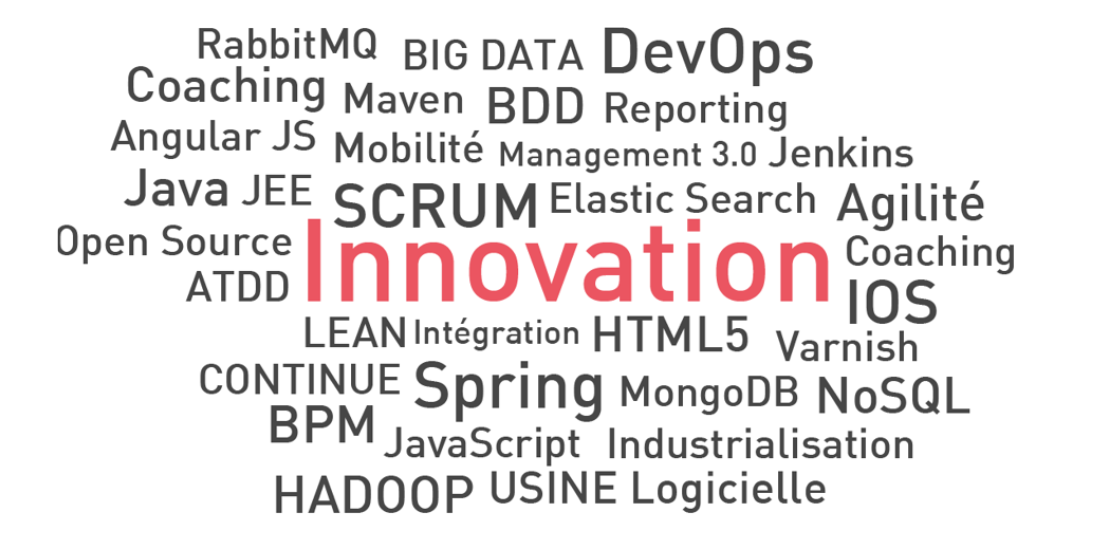
\includegraphics[keepaspectratio,width=\textwidth,height=0.75\textheight]{/Users/matekordial/Desktop/rapportstage2015/imagecatalogue.png}
Depuis sa création Zenika s’est positionnée sur les domaines technologiques qui font l’informatique de demain. Ce choix stratégique permet à la fois :

\begin{itemize}
\item d’offrir notre retour d’expérience, des formations, mais aussi de nombreux séminaires sur des domaines technologies de niches tout en conservant un positionnement sur les fondamentaux Java \slash JEE.

\item de recruter de manière sélective afin de sélectionner les meilleurs profils aptes à mener des projets qui n’ont en jamais été.

\end{itemize}

Pour cela, notre cellule de Direction Technique ; ainsi que l’ensemble de la communauté Zenika, effectue une veille technologique active, et participe à de nombreuses contributions open-source.

\begin{figure}[htbp]
\centering
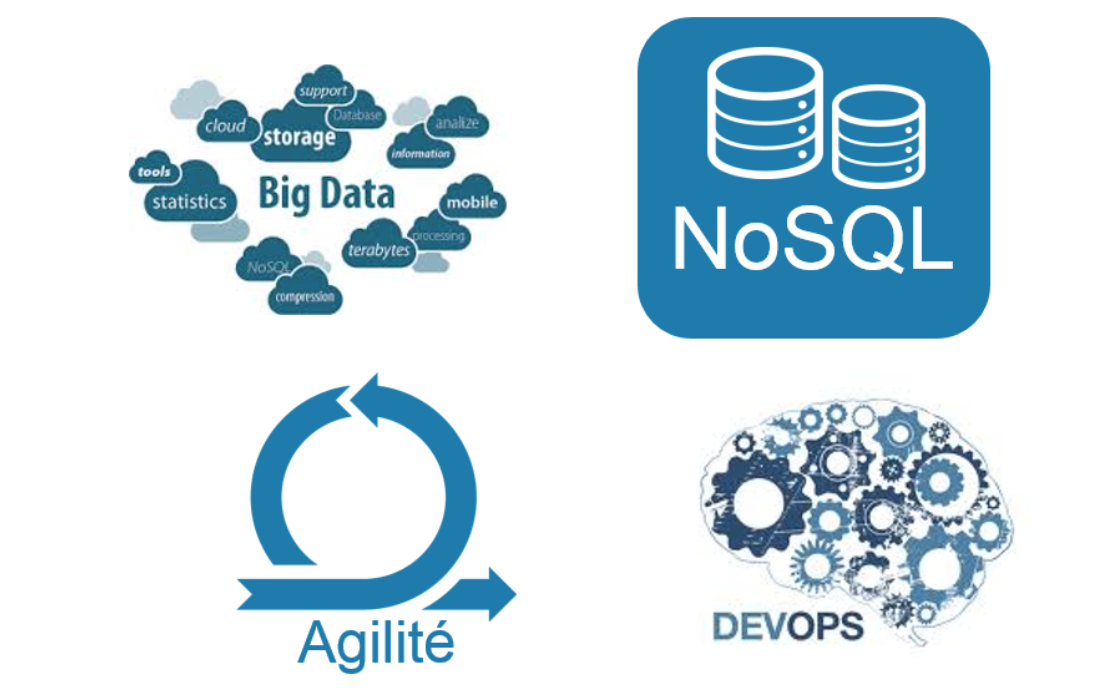
\includegraphics[keepaspectratio,width=\textwidth,height=0.75\textheight]{/Users/matekordial/Desktop/rapportstage2015/imageveille.png}
\caption{image}
\end{figure}

\subsection{Les compétences de l'entreprise}
\label{lescomptencesdelentreprise}

\begin{figure}[htbp]
\centering
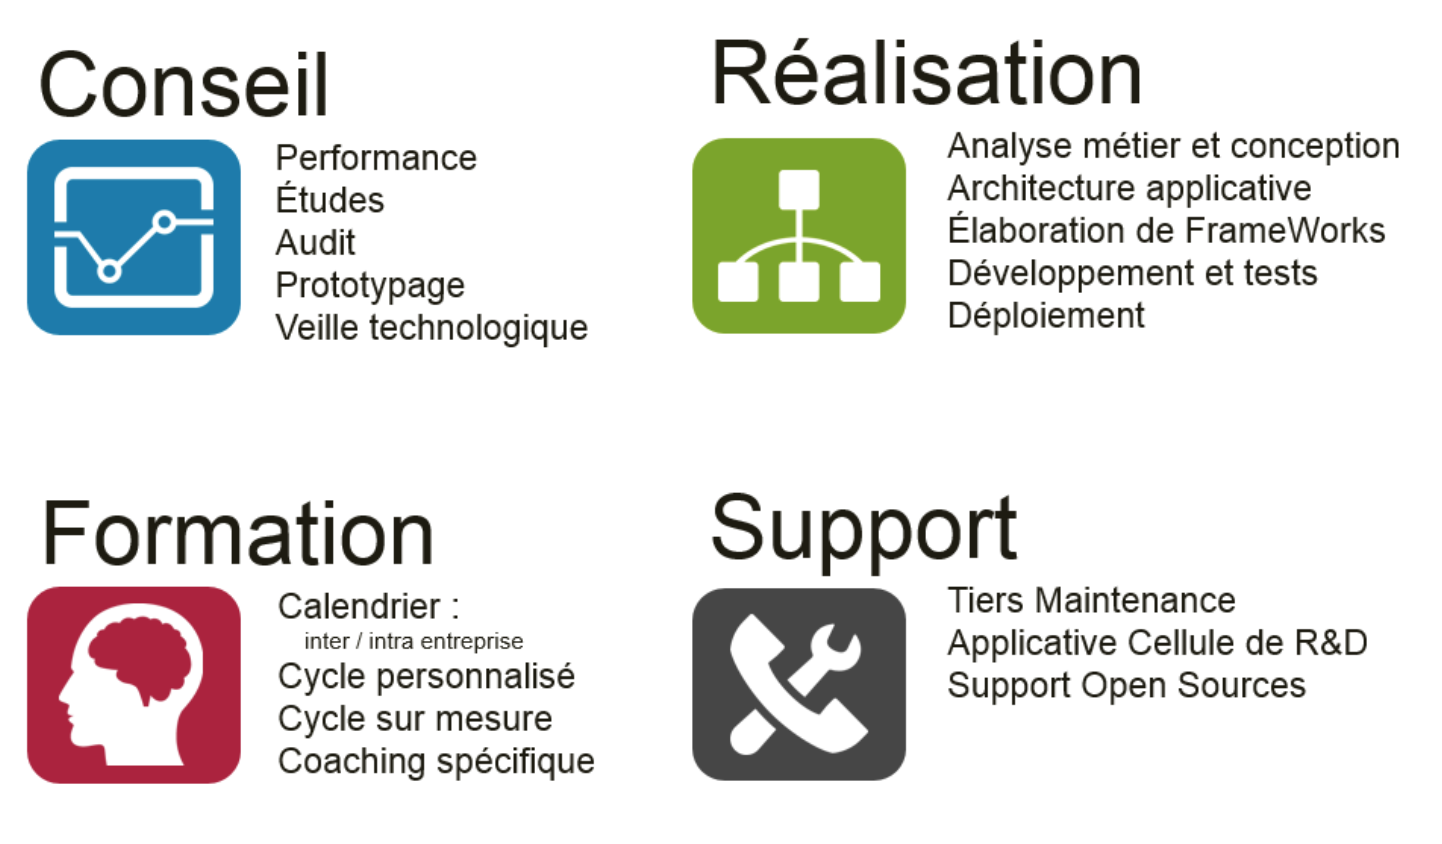
\includegraphics[keepaspectratio,width=\textwidth,height=0.75\textheight]{/Users/matekordial/Desktop/rapportstage2015/imagecompetence.png}
\caption{image}
\end{figure}

Les compétences de l'entreprise s'articulent autour de quatre grandes activités : \textbf{le conseil} , \textbf{la réalisation}, \textbf{la formation} et le \textbf{support}.

Les prinicipales domaines d'expertise de Zenika sont :

Le domaine d’expertise de Zenika va du Java débutant à Java spécialiste en passant par les nombreuses technologies de la boîte à outils java.



 

OpsDev est la vision DevOps de Zenika : une évolution culturelle du service informatique qui encourage la communication et la collaboration entre les équipes d’opérationnels (les Ops) et de développeurs
(les Devs), mais aussi les autres services (QA, DBA, Archi, Fonctionnels, Marketing, Commercial{\ldots}), dans le but de fournir des applications de meilleure qualité, plus fiable et répondant aux objectifs de la société.
Cette vision est l’extension logique de l’agilité à toute la chaîne de production des services informatiques.
Fort de son expérience agile et de son expertise technique tout autant Dev que Ops, Zenika propose de vous aider à construire votre démarche DevOps. 
 Alors que les projets confiés à la DSI sont toujours plus complexes, les approches prédictives historiques semblent toujours incapables d'y répondre.

De leur coté, les pratiques Agile permettent une augmentation de la satisfaction et de la qualité, tout en entraînant une réduction des délais et des coûts. 

 Le Craftsmanship, c’est quoi ?
« Le problème avec le ``vite et sale'', c'est que le ``sale'' demeure bien longtemps après que le ``vite'' ait été oublié. » - Steve McConnell

Apprenez à mettre votre code sous contôle, industrialisez votre environnement de travail, découvrez comment écrire du code de qualité. S’initier au craftsmanship n’est pas seulement une affaire d’experts, c’est aussi une affaire de passion. Chez Zenika, c’est notre ADN.
 La programmation ne se limite pas au backoffice. Zenika vous propose un pôle d’expertise complémentaire tourné front office tant sur des écrans génériques que sur des écrans mobiles.


 Allez au-delà de la business intelligence et développez vos outils décisionnels. A l’état de projet ou besoin de support, quel que soit le type de solution (colonnes, documents, clés\slash valeurs ou graph), nos experts peuvent vous apporter leur contribution. 

Zenika vous proposent du conseil, de la réalisation ou de la formation sur les technologies les plus performantes et innovantes.

\subsection{Zenika et La formation}
\label{zenikaetlaformation}

Zenika Training est un centre de formation agréé. Zenika profite de l'expertise de ses consultants pour faire monter en compétences à de nombreux développeurs sur toutes les technologies Open Source et les méthodes agiles. 

La formation constitue 25\% des chiffres d'affaires. Aujourd'hui, Zenika
 présente :

\begin{itemize}
\item Plus de 100 formations au catalogue

\item Llus de 15 formations officielles et certifiantes

\item Un important réseau de partenaires

\end{itemize}

\section{Les valeurs de l'entreprise}
\label{lesvaleursdelentreprise}

Zenika a été créé sur le modèle de l'entreprise dans laquelle les dirigeants aiméraient être lorsque nous étaient consultants : Une communauté d'experts partageant des valeurs humaines et techniques suivantes : \textbf{Transparence} /\slash  \textbf{Partage} /\slash  \textbf{Convivialité} 


 Conférences Open Source, animations internes, tables rondes{\ldots} sont autant d'occasions de partager vos connaissances techniques mais aussi vos idées, vos hobbies. Zenika vous donne la parole prenez-la !


 Réunions informelles, soirées thématiques, bubbles{\ldots} chaque occasion est propice aux échanges conviviaux.



\subsection{Les partenaires de l'entreprise}
\label{lespartenairesdelentreprise}

\begin{figure}[htbp]
\centering
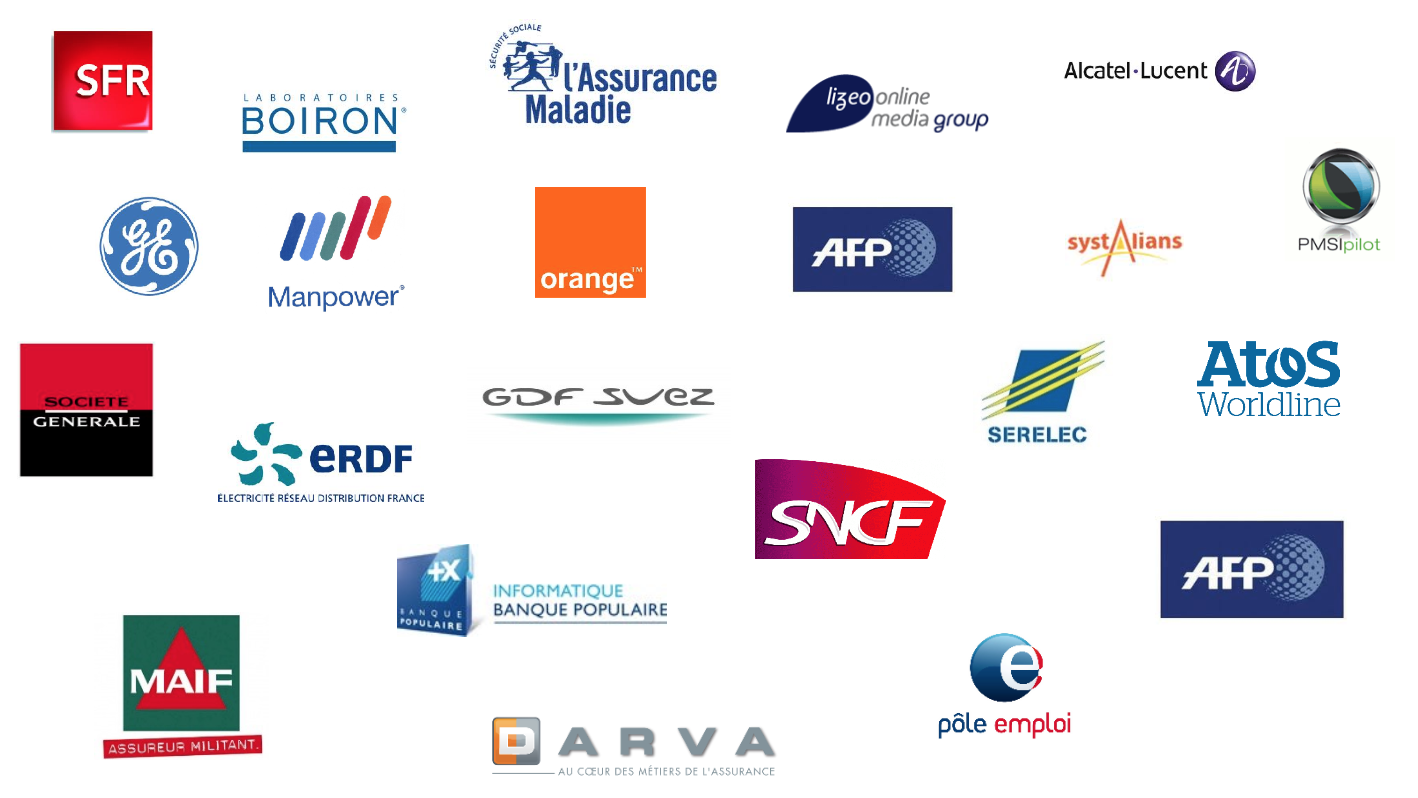
\includegraphics[keepaspectratio,width=\textwidth,height=0.75\textheight]{/Users/matekordial/Desktop/rapportstage2015/imagepartenaire.png}
\caption{image}
\end{figure}

\subsection{Zenika : Fiche de présentation détaillée}
\label{zenika:fichedeprsentationdtaille}

\begin{figure}[htbp]
\centering
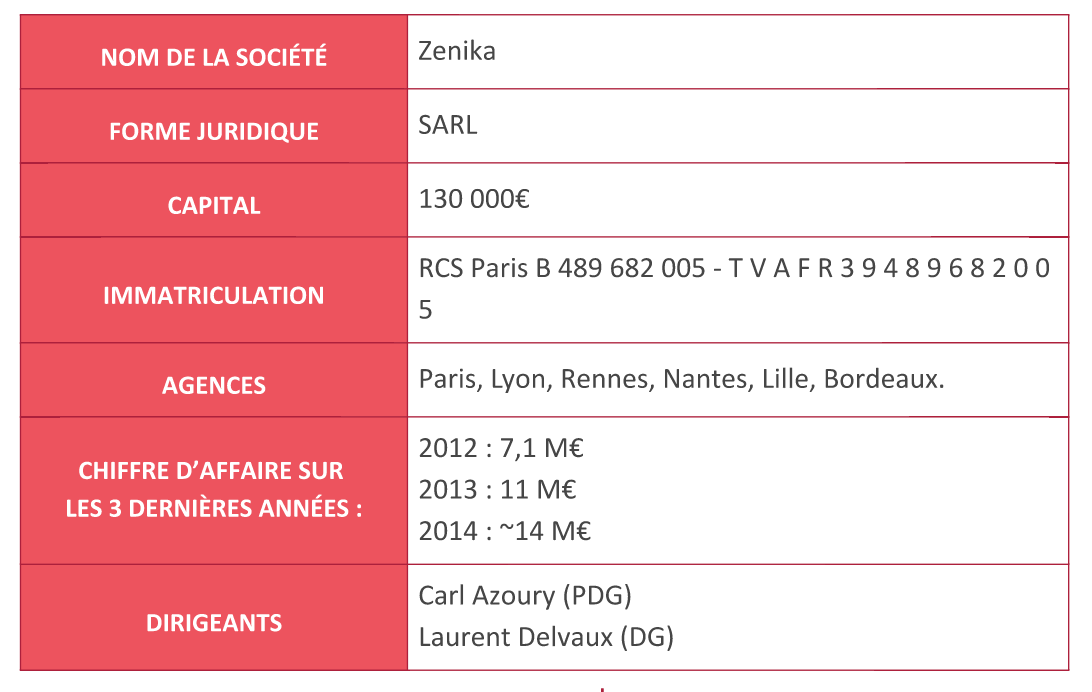
\includegraphics[keepaspectratio,width=\textwidth,height=0.75\textheight]{/Users/matekordial/Desktop/rapportstage2015/imagefiche.png}
\caption{image}
\end{figure}

\chapter{Presentation du travail}
\label{presentationdutravail}

\section{Presentation du sujet}
\label{presentationdusujet}

\subsubsection{Le but de stage}
\label{lebutdestage}

L'objectif de ce stage est de créer une plateforme multicanale à composantes, création de services en composition via interface web.

Pour expliquer le sujet avec des termes moins techniques, l'application devra permettre via une interface Web de créer une ressource en runtime en faisant un plug-play des différents composants.

\section{Le contexte}
\label{lecontexte}

Zenika Nord étant été créé en fin août 2014, il n'avait pas des locaux à Lille. De ce fait jusqu'au début de mon stage, les bureaux n'étaient pas prêts. L'achat et la contruction des locaux tout au long
 Ces locaux étant donc en construction, des bureaux provisoires ont été loués. La grande partie du stage s'est déroulé dans ces locaux provisoires. Les nouveaux locaux ont été finalement receptionnés en fin juillet.
 
 
 Concernant l'encadrement, j'étais sous la tutelle du directeur technique de Zenika Nord ,Gwennäel BUCHET. Nous organisons des rendez-vous hebdomadaires dans lequels nous faisions le point sur l'avancement du projet.

\section{Les aspects technologiques}
\label{lesaspectstechnologiques}

Durant ce stage j'ai eu l'occaion de pratiquer une large palette de technologies. Des technologies qui sont fortement appréciées par le monde des développeurs. Nous pouvons en citer : 
 Javassist (Java programming assistant ) rend la manipulation de bytecode Java simple. C' est une bibliothèque pour l'édition de bytecode en Java ; elle permet aux programmes Java de définir une nouvelle classe à l'exécution et de modifier une classe lorsque la JVM le charge . l'API Javassist offre deux niveaux : le niveau code source et le niveau bytecode . Si l'API est utilisé au niveau source , nous peuvons modifier un fichier code source d'une classe sans connaître les spécifications du bytecode Java . L' API est conçu avec seulement le vocabulaire du langage Java . Vous pouvez même spécifier le bytecode sous la forme d'un texte source et Javassist le compile à la volée . D'autre part , l' API au niveau bytecode permet aux utilisateurs d'éditer directement un fichier de classe .

 Spring est le framework de développement d'applications le plus populaire pour Java entreprises. Des millions de développeurs dans le monde utilisent Spring Framework pour créer du performant , facilement vérifiable , réutilisable code.

Spring Framework est une plate-forme Java open source et il a été initialement écrit par Rod Johnson et a d'abord été publié sous la licence Apache 2.0 en Juin de 2003.

Spring est léger par la taille. La version de base de Spring Framework est d'environ 2MB .

Les principaux éléments de Spring Framework peuvent être utilisés dans le développement de toute application Java, mais il existe des extensions pour construire des applications web au dessus de la plate-forme Java EE . Les objectifs de Spring Framework est de faciliter le développement d'applications J2EE et promouvoir les bonnes pratiques de programmation en permettant un modèle de programmation basé sur les POJO .

 Jersey Techniquement, les services REST sont spécifiés par le JCP (Java Community Process) sous le nom JAX-RS. Cette spécification précise ce que peut ou doit faire une implémentation, comme pour toutes ces spécifications. L'implémentation de référence que l'on utilise est Jersey. Jersey est installé en standard dans un serveur JEE (tel que Glassfish ou JBoss), et peut s'installer dans un serveur Tomcat.


 MongoDBest un système de base de données dans la mouvance NoSQL. Il est orienté documents. Son nom vient de Humongous qui veut dire énorme ou immense. L'objectif est donc de pouvoir gérer de grandes quantités de données. Comment ? Le moteur de base de données facilite l'extension (on parle de scaling) si bien que l'on pourra supporter l'accroissement de la quantité de données par l'ajout de machines.


 AngularJS
est un framework javascript qui permet de créer des application web dynamiques. Ce type d'applications (souvent appellées SPA pour
Single Page Application) sont de plus en plus présentes avec des périphériques connectés de plus en plus variés. Malheureusement, créer une application tenant sur une seule page n'est pas chose simple. En effet, cela requiert l'utilisation de beaucoup de javascript et il est très difficile de bien s'organiser et d'obtenir une application maintenable et modulable. Et c'est ici qu'AngularJS intervient.


\section{Le bilan}
\label{lebilan}

Le premier bilan à décompter de ce projet est d'être sûr que c'est possible de créer des ressources à la volée. Et cela permettait de surmonter de grandes difficutes en informatique. Celà permet de faire des appllciations multicanales. Par multicanales nous pouvons entendre, des applications adaptables selon les types de canaux utilisés (ordinateur, tablettes, smartphones etc {\ldots}).

\subsection{Vérifier la faisaibilité du projet.}
\label{vrifierlafaisaibilitduprojet.}

Avant de se lancer et se rendre trois mois plus tard que le projet n'était pas faisable, nous avions jugé important de vérifier la faisaibilité au niveau technologies de projet. 

Ainsi il y avait cinq difficultés majeures que nous devions surmonter . Nous avons décidé de les appeler des challenges pour qu'elles ne soient pas des obstacles pour nous. Les principales questions posées étaient : 

\begin{itemize}
\item Est il possible de générer des ressources à la volée ?

\item Etant donné que le serveur était déjà démarré, Est il possible de loader ces ressources générées avec Jersey?

\item Spring pourrait il re-scanner ces ressources ?

\end{itemize}

Pour vérifier la faisabilité du projet, nous avons créé pour chaque difficulté un \textbf{poc} pour tester avec quelle technologie nous pouvions la surmonter.

Un \textbf{poc} ( Proof of concept en anglais ) est étape de valdation concrète dans la mise en place d'un projet radicalement nouveau. C'est un projet jetable destiner à mesurer la faisabilité et le niveau de difficulté du projet.

Ces pocs nous ont permis d'avoir des solutions techniques aux problèmes posés.

Pour la première difficulté, nous avons trouvé aprés moult recherches Javassist qui est un Framework qui permet de générer des classes et permet aussi d'ajouter des annotations à ces classes. Donc cela resolvait notre probléme car une resource n'est rien d'autre qu'une classe avec des annotations.

Pour la deuxième difficulté, nous avons découvert qu'il suffisait juste d'utiliser la fonction \textbf{register} de Jersey dans une methode avec l'annotation \textbf{@PostContruct} pour que Jersey reconnait la nouvelle resource générée.

Il s'est trouvé que nous avions même pas besoin de rescanner les ressources pour que Spring puisse prendre en compte cette nouvelle ressource. Il suffisait qu'elle soit générée et registrée pour que Spring le reconnait.

\subsubsection{Etapes de développement}
\label{etapesdedveloppement}

\section{Les perspectives.}
\label{lesperspectives.}

\chapter{Le bilan personnel du stage.}
\label{lebilanpersonneldustage.}
\end{document}